\documentclass{beamer}
\usepackage{listings}
\usetheme{Copenhagen}
\usecolortheme{beaver}
\setbeamertemplate{navigation symbols}{}
\setbeamertemplate{footline}{\parbox[t][12pt][c]{12pt}{~\scriptsize\insertframenumber}}
% \usepackage{beamerthemesplit} // Activate for custom appearance

\title{Declarative Cartography}
\subtitle{In-Database Map Generalization of Spatial Datasets}
\author{\underline{Pimin Konstantin Kefaloukos}, Marcos Vaz Salles, Martin Zachariasen\\ \small{Computer Science Department, University of Copenhagen} (DIKU)}
\date{\today}

\begin{document}

\frame{\titlepage}

% MOTIVATION
\frame
{
  \frametitle{Overview}
  \begin{center}
  \fbox{A narrow view of the world of digital web maps :-)}
  \end{center}
  
  \begin{itemize}
  \item \textbf{OK}: Background maps are stable and of good quality (commercial and national map providers)
  \item \textbf{Work needed}: Foreground data is dynamic and constantly emerging and changing (social media, sensors, ...)
  \item \textbf{Challenge}: Design \emph{easy-to-use}, \emph{cheap}, \emph{scalable} and \emph{effective} method for \underline{generalizing}, \underline{serving} and \underline{visualizing} foreground data
  \item \textbf{Use cases}: Data journalism, citizen information systems, crisis response, social media, ...
  \end{itemize}

}

\frame
{
  \frametitle{Our approach}
  \begin{itemize}
  \item \textbf{Language}: Design and implement an easy to use \emph{programming language} for generalizing spatial data 
  \item \textbf{Optimization}: Fit generalization problem to well-known \emph{optimization problem}, i.e. variant of Set Cover Problem~\cite{vazirani}
  \item \textbf{Algorithms}: Reuse \emph{existing algorithms} for this problem
  \item \textbf{Databases}: Reuse \emph{database technology} and \emph{move code to data} by implementing algorithms in a spatial database
  \end{itemize}
  \begin{center}
  \fbox{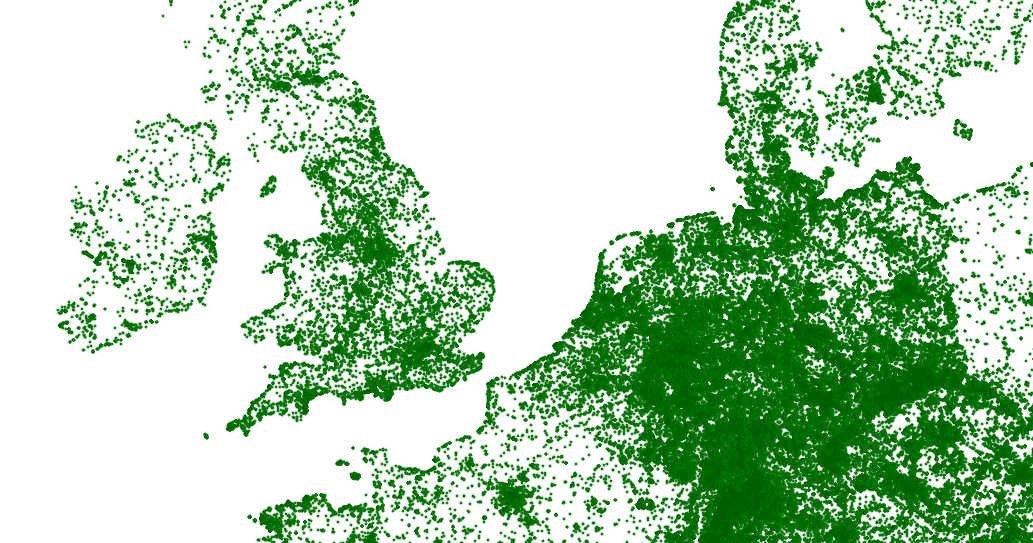
\includegraphics[scale=0.18]{figs/toomanyobjects.png}}
  \end{center}
}

\frame
{
  \frametitle{Relation to Reverse Data Management}

  We implemented \emph{how-to} queries for spatial data:
  \begin{itemize}
  \item \textbf{How-to queries}~\cite{reversedatamanagement}: Given an \emph{input database}; compute an \emph{output database}, subject to set of \emph{constraints} and minimizing/maximizing an \emph{objective function}
  \item \textbf{Spatial example}: Given an \emph{input database of spatial objects}; compute an output database that generalizes the objects to $\mathcal{Z}$ zoom-levels, subject to \emph{spatial constraints} and while \emph{minimizing loss} of objects in map (with prioritization)
  \end{itemize}
}

\frame
{
  \frametitle{Please note!}
  When you see the word \emph{``delete''} in this presentation, please append the words \emph{``or aggregate (future work)''} in your mind. \\
  making grammatical adjustments where appropriate.
  
  \begin{center}
  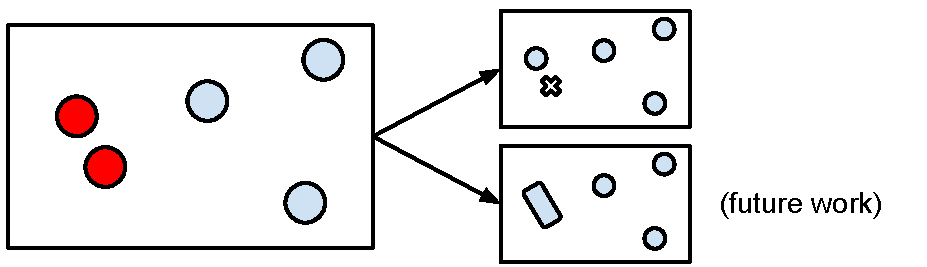
\includegraphics[scale=0.50]{figs/cvl-delete-aggregate.pdf}
  \end{center}

}


\frame
{
  \frametitle{Problem definition}
  \begin{itemize}
  \item Spatial objects with \emph{unique ID}, \emph{weight} and \emph{geometry} (point, linestring, polygon etc)
  \item Compute minimum zoom-level for all objects:
  \begin{itemize}
  \item Minimize weight of objects that are missing
  \item Subject to spatial constraints (proximity, density, ...)
  \end{itemize}
  \end{itemize}
  \begin{center}
  \fbox{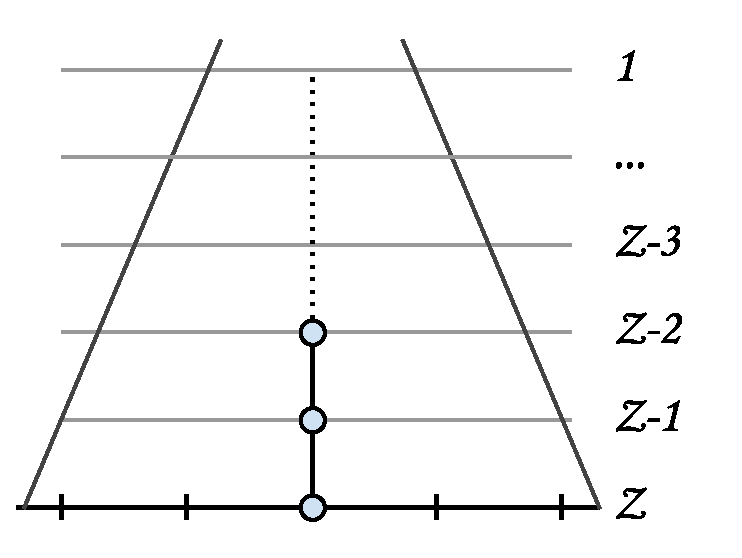
\includegraphics[scale=0.4]{figs/cvl-problem.pdf}}
  \end{center}
}

\frame
{
  \frametitle{Constraints}

  \begin{itemize}
  \item \textbf{Zoom-consistency} If object in missing from zoom-level, it is also missing from all lower zoom-levels~\cite{fusiontables}
  \item \textbf{User-defined constraints}:
  \begin{itemize}
  \item Arbitrary property that must hold for \emph{sets of objects}
  \item If property does not hold for set of objects $\implies$ \emph{conflict}
  \item Conflicts resolved by \emph{deleting} objects
  \item Example: \emph{proximity}
  \end{itemize}
  \end{itemize}
  
  \begin{center}
  	\fbox{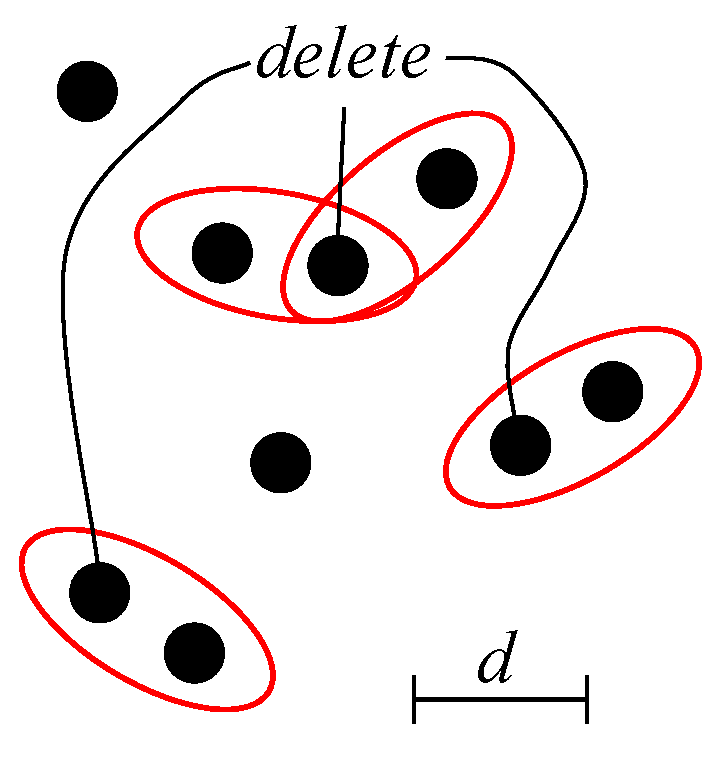
\includegraphics[scale=0.20]{figs/cvl-proximity-conflicts-2.pdf}} \fbox{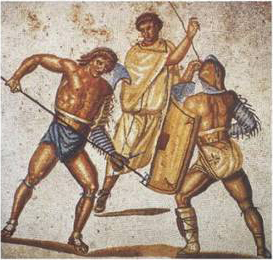
\includegraphics[scale=.38]{figs/gladiators.jpg}} \fbox{
\includegraphics[scale=.288]{figs/the-godfather-1.jpg}}
  \end{center}
  
    \begin{itemize}
  \item Like a gladiator fight, but outcome is decided by ``management''
  \end{itemize}

}

\frame
{
  \frametitle{Constraints: Proximity}
  \textbf{Proximity constraint}:
  \begin{itemize}
  \item Any two objects must be separated by minimum distance
  \item Resolve conflicts by deleting one object
  \end{itemize}
  \begin{center}
  \fbox{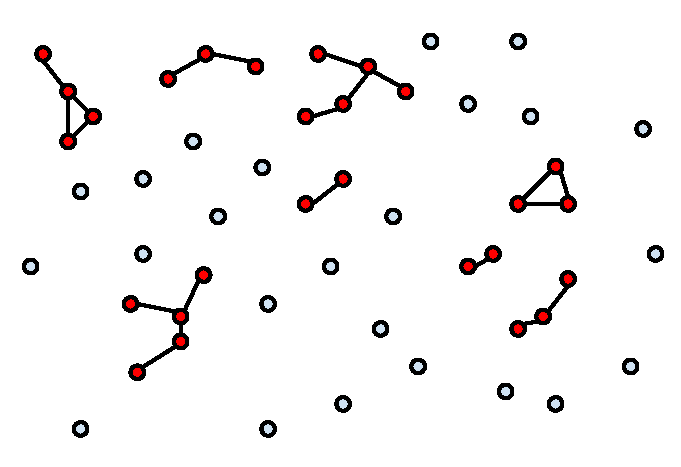
\includegraphics[scale=0.4]{figs/cvl-proximity.pdf}} \\
  \small{Red objects violate proximity constraint}
  \end{center}
}

\frame
{
  \frametitle{Constraints: Visibility}
  \textbf{Visibility constraint}:  
  \begin{itemize}
  \item Within unit area, at most $K$ objects may be visible
  \item Resolve conflict (involving $K'$ objects) by deleting $K' - K$ objects
  \end{itemize}
  \begin{center}
  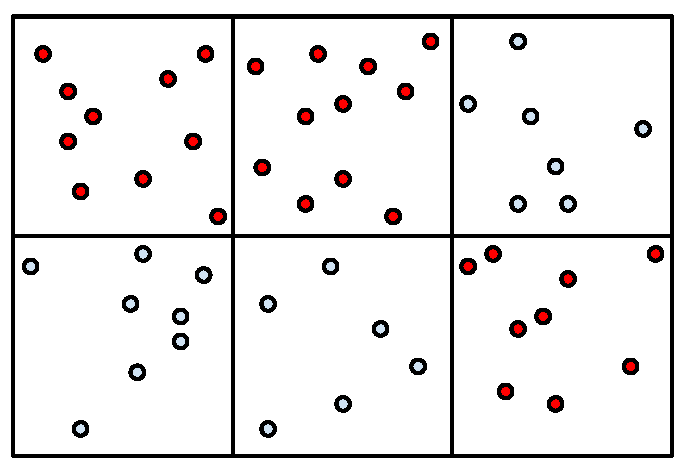
\includegraphics[scale=0.4]{figs/cvl-visibility.pdf} \\
  \small{Red objects violate visibility constraint ($K=8$)}
  \end{center}
}

\frame
{
  \frametitle{Future work}
  \begin{itemize}
  \item Relax zoom-consistency: \emph{min} and \emph{max} zoom-level for records)
  \item Extend work with \emph{aggregation} in language (semantics) and algorithm (implementation)
  \item Implement compilation of CVL to a distributed database dialect
  \end{itemize}
}

\frame
{
  \frametitle{Future work: Aggregation}
  \begin{center}
  \fbox{This is where I really need your help :-)}
  \end{center}

  \begin{itemize}
  \item \textbf{User-level semantics}:
  \begin{itemize}
  \item How should user \emph{understand} aggregation, e.g. aggregation of non-geometric attributes?
  \item How should user \emph{parameterize} aggregation?
  \end{itemize}
  \item \textbf{Implementation}:
  \begin{itemize}
  \item Can we \emph{stretch} the existing model to include aggregation?
  \item Else, how does aggregation \emph{change} the problem/model?
  \item Do we need new \emph{algorithms}?
  \end{itemize}
  \end{itemize}

  \begin{center}
  \fbox{\textbf{Eiffel Tower + Louvre = ?}}
  \end{center}

}



% RELATED WORK
\frame
{
  \frametitle{Related work}

  \begin{itemize}
  \item \emph{Efficient Spatial Sampling of Large Geographical Tables}. Das Sarma, A., Lee, H., Gonzalez, H., Madhavan, J., \& Halevy, A. (2012).
  \item \emph{Reverse data management}, Meliou, A., Gatterbauer, W., \& Suciu, D. (2011).
  \item \emph{Generalization of land cover maps by mixed integer programming}. Haunert, J.-H., \& Wolff, A. (2006). 
  \item \emph{Constant information density in zoomable interfaces}. Woodruff, A., Landay, J., Stonebraker, M. (1998).
  \item And tons more of course...
  \end{itemize}
}

% Past and future work
\frame
{
  \frametitle{Past and future work}

  \begin{itemize}
  \item Past work: \emph{TileHeat}, predicting where people will look on a map tomorrow
  \item Latest work: \emph{Declarative Cartography}, the work described in these slides
  \item Future work: \emph{Real-time Declarative Cartography}, joint work with people at University of Zurich (Department of Geography)
  \item Future work: Succinct data representation of high-fidelity spatial data that is visualized on a digital map on a screen (think: pixel precision is not all that good)
  \end{itemize}
}




\end{document}
